\PassOptionsToPackage{unicode=true}{hyperref} % options for packages loaded elsewhere
\PassOptionsToPackage{hyphens}{url}
%
\documentclass[]{article}
\usepackage{lmodern}
\usepackage{amssymb,amsmath}
\usepackage{ifxetex,ifluatex}
\usepackage{fixltx2e} % provides \textsubscript
\ifnum 0\ifxetex 1\fi\ifluatex 1\fi=0 % if pdftex
  \usepackage[T1]{fontenc}
  \usepackage[utf8]{inputenc}
  \usepackage{textcomp} % provides euro and other symbols
\else % if luatex or xelatex
  \usepackage{unicode-math}
  \defaultfontfeatures{Ligatures=TeX,Scale=MatchLowercase}
\fi
% use upquote if available, for straight quotes in verbatim environments
\IfFileExists{upquote.sty}{\usepackage{upquote}}{}
% use microtype if available
\IfFileExists{microtype.sty}{%
\usepackage[]{microtype}
\UseMicrotypeSet[protrusion]{basicmath} % disable protrusion for tt fonts
}{}
\IfFileExists{parskip.sty}{%
\usepackage{parskip}
}{% else
\setlength{\parindent}{0pt}
\setlength{\parskip}{6pt plus 2pt minus 1pt}
}
\usepackage{hyperref}
\hypersetup{
            pdftitle={Bootstrap - Interactions and Seeds},
            pdfauthor={SDS 291},
            pdfborder={0 0 0},
            breaklinks=true}
\urlstyle{same}  % don't use monospace font for urls
\usepackage[margin=1in]{geometry}
\usepackage{color}
\usepackage{fancyvrb}
\newcommand{\VerbBar}{|}
\newcommand{\VERB}{\Verb[commandchars=\\\{\}]}
\DefineVerbatimEnvironment{Highlighting}{Verbatim}{commandchars=\\\{\}}
% Add ',fontsize=\small' for more characters per line
\usepackage{framed}
\definecolor{shadecolor}{RGB}{248,248,248}
\newenvironment{Shaded}{\begin{snugshade}}{\end{snugshade}}
\newcommand{\AlertTok}[1]{\textcolor[rgb]{0.94,0.16,0.16}{#1}}
\newcommand{\AnnotationTok}[1]{\textcolor[rgb]{0.56,0.35,0.01}{\textbf{\textit{#1}}}}
\newcommand{\AttributeTok}[1]{\textcolor[rgb]{0.77,0.63,0.00}{#1}}
\newcommand{\BaseNTok}[1]{\textcolor[rgb]{0.00,0.00,0.81}{#1}}
\newcommand{\BuiltInTok}[1]{#1}
\newcommand{\CharTok}[1]{\textcolor[rgb]{0.31,0.60,0.02}{#1}}
\newcommand{\CommentTok}[1]{\textcolor[rgb]{0.56,0.35,0.01}{\textit{#1}}}
\newcommand{\CommentVarTok}[1]{\textcolor[rgb]{0.56,0.35,0.01}{\textbf{\textit{#1}}}}
\newcommand{\ConstantTok}[1]{\textcolor[rgb]{0.00,0.00,0.00}{#1}}
\newcommand{\ControlFlowTok}[1]{\textcolor[rgb]{0.13,0.29,0.53}{\textbf{#1}}}
\newcommand{\DataTypeTok}[1]{\textcolor[rgb]{0.13,0.29,0.53}{#1}}
\newcommand{\DecValTok}[1]{\textcolor[rgb]{0.00,0.00,0.81}{#1}}
\newcommand{\DocumentationTok}[1]{\textcolor[rgb]{0.56,0.35,0.01}{\textbf{\textit{#1}}}}
\newcommand{\ErrorTok}[1]{\textcolor[rgb]{0.64,0.00,0.00}{\textbf{#1}}}
\newcommand{\ExtensionTok}[1]{#1}
\newcommand{\FloatTok}[1]{\textcolor[rgb]{0.00,0.00,0.81}{#1}}
\newcommand{\FunctionTok}[1]{\textcolor[rgb]{0.00,0.00,0.00}{#1}}
\newcommand{\ImportTok}[1]{#1}
\newcommand{\InformationTok}[1]{\textcolor[rgb]{0.56,0.35,0.01}{\textbf{\textit{#1}}}}
\newcommand{\KeywordTok}[1]{\textcolor[rgb]{0.13,0.29,0.53}{\textbf{#1}}}
\newcommand{\NormalTok}[1]{#1}
\newcommand{\OperatorTok}[1]{\textcolor[rgb]{0.81,0.36,0.00}{\textbf{#1}}}
\newcommand{\OtherTok}[1]{\textcolor[rgb]{0.56,0.35,0.01}{#1}}
\newcommand{\PreprocessorTok}[1]{\textcolor[rgb]{0.56,0.35,0.01}{\textit{#1}}}
\newcommand{\RegionMarkerTok}[1]{#1}
\newcommand{\SpecialCharTok}[1]{\textcolor[rgb]{0.00,0.00,0.00}{#1}}
\newcommand{\SpecialStringTok}[1]{\textcolor[rgb]{0.31,0.60,0.02}{#1}}
\newcommand{\StringTok}[1]{\textcolor[rgb]{0.31,0.60,0.02}{#1}}
\newcommand{\VariableTok}[1]{\textcolor[rgb]{0.00,0.00,0.00}{#1}}
\newcommand{\VerbatimStringTok}[1]{\textcolor[rgb]{0.31,0.60,0.02}{#1}}
\newcommand{\WarningTok}[1]{\textcolor[rgb]{0.56,0.35,0.01}{\textbf{\textit{#1}}}}
\usepackage{graphicx,grffile}
\makeatletter
\def\maxwidth{\ifdim\Gin@nat@width>\linewidth\linewidth\else\Gin@nat@width\fi}
\def\maxheight{\ifdim\Gin@nat@height>\textheight\textheight\else\Gin@nat@height\fi}
\makeatother
% Scale images if necessary, so that they will not overflow the page
% margins by default, and it is still possible to overwrite the defaults
% using explicit options in \includegraphics[width, height, ...]{}
\setkeys{Gin}{width=\maxwidth,height=\maxheight,keepaspectratio}
\setlength{\emergencystretch}{3em}  % prevent overfull lines
\providecommand{\tightlist}{%
  \setlength{\itemsep}{0pt}\setlength{\parskip}{0pt}}
\setcounter{secnumdepth}{0}
% Redefines (sub)paragraphs to behave more like sections
\ifx\paragraph\undefined\else
\let\oldparagraph\paragraph
\renewcommand{\paragraph}[1]{\oldparagraph{#1}\mbox{}}
\fi
\ifx\subparagraph\undefined\else
\let\oldsubparagraph\subparagraph
\renewcommand{\subparagraph}[1]{\oldsubparagraph{#1}\mbox{}}
\fi

% set default figure placement to htbp
\makeatletter
\def\fps@figure{htbp}
\makeatother


\title{Bootstrap - Interactions and Seeds}
\author{SDS 291}
\date{March 4, 2020}

\begin{document}
\maketitle

Two things about the bootstrap for homeworks:

\begin{enumerate}
\def\labelenumi{\arabic{enumi}.}
\item
  The bootstrap will take a different sample every time - and you'll get
  different answers. The solution is to \emph{set a seed} so that every
  time you knit the file, you will start in the same place, get the same
  distribution, and thus get the same answer.
\item
  Also, it's better practice to \emph{knit your whole file over and over
  again} rather than running code chunks iteratively so that you
  minimize discrepancies between the answers from your knitted verson
  with one seed and the answers you got when running the code in a code
  chunk that used a different seed.
\item
  Naming conventions for interaction terms differ between how the
  coefficient is saved from a regression model and how it's saved in the
  bootstrap distribution
\end{enumerate}

\hypertarget{set-the-seed}{%
\section{Set the Seed}\label{set-the-seed}}

I'm going to set the seed at the beginning, in the code chunk below.

\begin{Shaded}
\begin{Highlighting}[]
\NormalTok{knitr}\OperatorTok{::}\NormalTok{opts_chunk}\OperatorTok{$}\KeywordTok{set}\NormalTok{(}\DataTypeTok{echo =} \OtherTok{TRUE}\NormalTok{)}
\KeywordTok{require}\NormalTok{(Stat2Data)}
\KeywordTok{require}\NormalTok{(mosaic)}
\KeywordTok{require}\NormalTok{(magrittr)}
\KeywordTok{require}\NormalTok{(tidyverse)}
\KeywordTok{data}\NormalTok{(}\StringTok{"FirstYearGPA"}\NormalTok{)}

\KeywordTok{set.seed}\NormalTok{(}\DecValTok{8675309}\NormalTok{)}
\end{Highlighting}
\end{Shaded}

The seed can be any number -- today's date, your birthday, your
telephone number, your zipcode -- and R will be consistent when creating
the bootstrap sample to pick the same starting point for resampling.
It's an abstract concept, which is why the seed doesn't actually need to
be, say, a number in the dataset.

\hypertarget{fit-the-regression-equation}{%
\subsection{Fit the regression
equation}\label{fit-the-regression-equation}}

Fit the simple linear regression equation
\(GPA=\beta_0+\beta_1 SATM + \beta_2 HSGPA+ \beta_3 (SATM \times HSGPA) + \epsilon\)
and construct a 95\% CI for the estimate for \(\beta_3\). {[}Hint:
Remember that you can use \texttt{confint()} to calculate the 95\% CI
for all terms in the model (put the name of the model in the
parentheses){]}.

\begin{Shaded}
\begin{Highlighting}[]
\NormalTok{SATM_orig<-}\KeywordTok{lm}\NormalTok{(GPA}\OperatorTok{~}\NormalTok{SATM}\OperatorTok{*}\NormalTok{HSGPA, }\DataTypeTok{data=}\NormalTok{FirstYearGPA)}
\KeywordTok{summary}\NormalTok{(SATM_orig)}
\end{Highlighting}
\end{Shaded}

\begin{verbatim}
## 
## Call:
## lm(formula = GPA ~ SATM * HSGPA, data = FirstYearGPA)
## 
## Residuals:
##      Min       1Q   Median       3Q      Max 
## -1.00571 -0.31168  0.05113  0.30683  0.82901 
## 
## Coefficients:
##               Estimate Std. Error t value Pr(>|t|)
## (Intercept)  1.4644149  2.3415700   0.625    0.532
## SATM        -0.0003161  0.0036773  -0.086    0.932
## HSGPA        0.3235961  0.6833125   0.474    0.636
## SATM:HSGPA   0.0003258  0.0010693   0.305    0.761
## 
## Residual standard error: 0.4149 on 215 degrees of freedom
## Multiple R-squared:  0.2163, Adjusted R-squared:  0.2054 
## F-statistic: 19.78 on 3 and 215 DF,  p-value: 2.315e-11
\end{verbatim}

\begin{Shaded}
\begin{Highlighting}[]
\KeywordTok{confint}\NormalTok{(SATM_orig)}
\end{Highlighting}
\end{Shaded}

\begin{verbatim}
##                    2.5 %      97.5 %
## (Intercept) -3.150958000 6.079787785
## SATM        -0.007564155 0.006932016
## HSGPA       -1.023253163 1.670445334
## SATM:HSGPA  -0.001781796 0.002433416
\end{verbatim}

You'll note that here the coefficient from the model SATM\_orig is saved
as \texttt{SATM:HSGPA} (with a colon). This becomes important later,
because it gets saved with a different name in the bootstrap
distribution that you will calculate below.

\hypertarget{construct-the-bootstrap-distribution-for-regression-coefficients}{%
\subsection{Construct the Bootstrap Distribution for Regression
Coefficients}\label{construct-the-bootstrap-distribution-for-regression-coefficients}}

Construct the bootstrap distribution by estimating the coefficients from
the regression model (i.e., the bootstrap statistic) in 5000 bootstrap
samples. Make a histogram of the bootstrap distribution of the slope
coefficient for SATM.

\begin{Shaded}
\begin{Highlighting}[]
\NormalTok{SATM_bootstrap<-}\StringTok{ }\KeywordTok{do}\NormalTok{(}\DecValTok{5000}\NormalTok{) }\OperatorTok{*}\StringTok{ }\KeywordTok{coef}\NormalTok{(}\KeywordTok{lm}\NormalTok{(GPA}\OperatorTok{~}\NormalTok{SATM}\OperatorTok{*}\NormalTok{HSGPA, }\DataTypeTok{data=}\KeywordTok{resample}\NormalTok{(FirstYearGPA)))}
\KeywordTok{glimpse}\NormalTok{(SATM_bootstrap)}
\end{Highlighting}
\end{Shaded}

\begin{verbatim}
## Observations: 5,000
## Variables: 4
## $ Intercept  <dbl> 7.31351325, 1.15982443, 2.73081168, -2.43560764, 3.30632...
## $ SATM       <dbl> -0.0092813434, 0.0005795890, -0.0027062226, 0.0055896367...
## $ HSGPA      <dbl> -1.33312407, 0.49189724, -0.10490374, 1.40107312, -0.232...
## $ SATM.HSGPA <dbl> 2.847030e-03, -5.476726e-05, 1.100933e-03, -1.332998e-03...
\end{verbatim}

\begin{Shaded}
\begin{Highlighting}[]
\KeywordTok{qplot}\NormalTok{(}\DataTypeTok{x=}\NormalTok{SATM.HSGPA, }\DataTypeTok{data=}\NormalTok{SATM_bootstrap)}
\end{Highlighting}
\end{Shaded}

\begin{verbatim}
## `stat_bin()` using `bins = 30`. Pick better value with `binwidth`.
\end{verbatim}

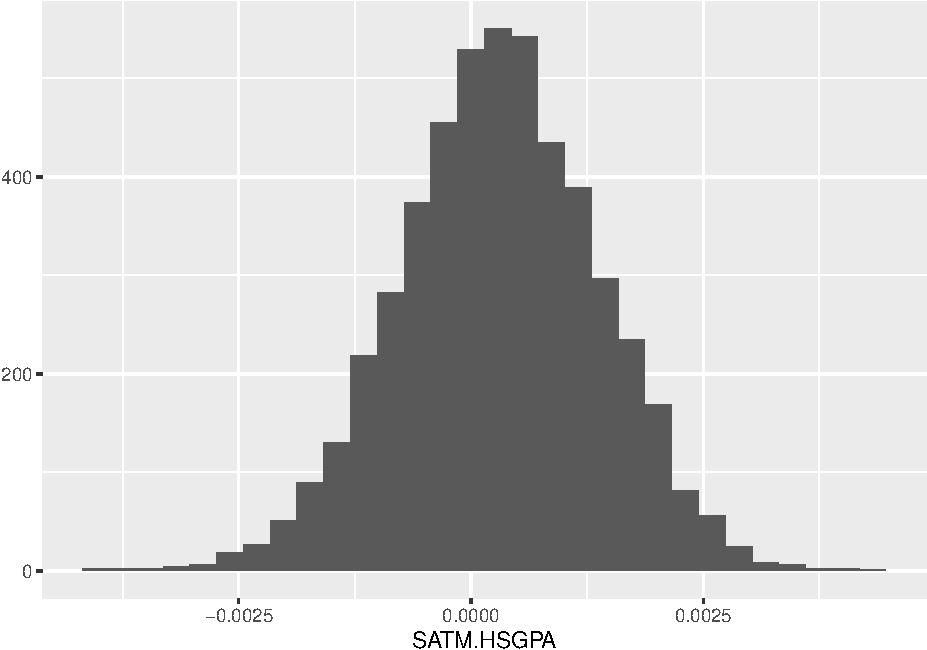
\includegraphics{Day12_InClassLab_Answers_files/figure-latex/unnamed-chunk-3-1.pdf}

Here, you'll notice that the interaction term is called
\texttt{SATM.HSGPA} in the bootstrap distribution. Now we have different
values about the interaction term saved with different names in two
different places.

So, when we wan't to use the coefficient from the original regression
(like in Methods 1 and 3), we'll need to use
\texttt{coef(SATM\_orig){[}"SATM:HSGPA"{]}} and when we want values from
the bootstrap distribution to calculate the standard error or quantiles
around of the bootstrap distribution, the value is called
\texttt{SATM.HSGPA} from the \texttt{SATM\_bootstrap} dataset we just
built above.

\hypertarget{confidence-intervals}{%
\subsection{Confidence Intervals}\label{confidence-intervals}}

Estimate the CI with each of the three approaches and compare them at
the end.

\hypertarget{method-1-standard-deviation}{%
\subsubsection{Method 1: Standard
Deviation}\label{method-1-standard-deviation}}

\begin{Shaded}
\begin{Highlighting}[]
\NormalTok{zs <-}\StringTok{ }\KeywordTok{qnorm}\NormalTok{(}\KeywordTok{c}\NormalTok{(}\FloatTok{0.025}\NormalTok{, }\FloatTok{0.975}\NormalTok{))}
\KeywordTok{coef}\NormalTok{(SATM_orig)[}\StringTok{"SATM:HSGPA"}\NormalTok{] }\OperatorTok{+}\StringTok{ }\NormalTok{zs }\OperatorTok{*}\StringTok{ }\KeywordTok{sd}\NormalTok{(}\OperatorTok{~}\NormalTok{SATM.HSGPA, }\DataTypeTok{data=}\NormalTok{SATM_bootstrap)}
\end{Highlighting}
\end{Shaded}

\begin{verbatim}
## [1] -0.001782178  0.002433798
\end{verbatim}

\hypertarget{method-2---quantiles-from-the-bootstrap-distribution}{%
\subsubsection{Method \#2 - Quantiles from the Bootstrap
Distribution}\label{method-2---quantiles-from-the-bootstrap-distribution}}

\begin{Shaded}
\begin{Highlighting}[]
\KeywordTok{qdata}\NormalTok{(}\OperatorTok{~}\NormalTok{SATM.HSGPA, }\DataTypeTok{p=}\KeywordTok{c}\NormalTok{(}\FloatTok{0.025}\NormalTok{, }\FloatTok{0.975}\NormalTok{), }\DataTypeTok{data=}\NormalTok{SATM_bootstrap)}
\end{Highlighting}
\end{Shaded}

\begin{verbatim}
##           quantile     p
## 2.5%  -0.001846888 0.025
## 97.5%  0.002353318 0.975
\end{verbatim}

\hypertarget{method-3---reverse-the-quantiles-from-the-bootstrap-distribution}{%
\subsubsection{Method \#3 - Reverse the quantiles from the bootstrap
distribution}\label{method-3---reverse-the-quantiles-from-the-bootstrap-distribution}}

\begin{Shaded}
\begin{Highlighting}[]
\NormalTok{qs <-}\StringTok{ }\KeywordTok{qdata}\NormalTok{(}\OperatorTok{~}\NormalTok{SATM.HSGPA, }\DataTypeTok{p =} \KeywordTok{c}\NormalTok{(}\FloatTok{0.025}\NormalTok{, }\FloatTok{0.975}\NormalTok{), }\DataTypeTok{data=}\NormalTok{SATM_bootstrap)}\OperatorTok{$}\NormalTok{quantile}
\KeywordTok{coef}\NormalTok{(SATM_orig)[}\StringTok{"SATM:HSGPA"}\NormalTok{] }\OperatorTok{-}\StringTok{ }\NormalTok{(qs }\OperatorTok{-}\StringTok{ }\KeywordTok{coef}\NormalTok{(SATM_orig)[}\StringTok{"SATM:HSGPA"}\NormalTok{])}
\end{Highlighting}
\end{Shaded}

\begin{verbatim}
## [1]  0.002498509 -0.001701698
\end{verbatim}

\end{document}
